\section{UC2--UC3: Project and Member Management}

\clearpage
\begin{landscape}
\thispagestyle{landscapefancy}
\begin{figure}[H]
\centering
\makebox[\linewidth][c]{%
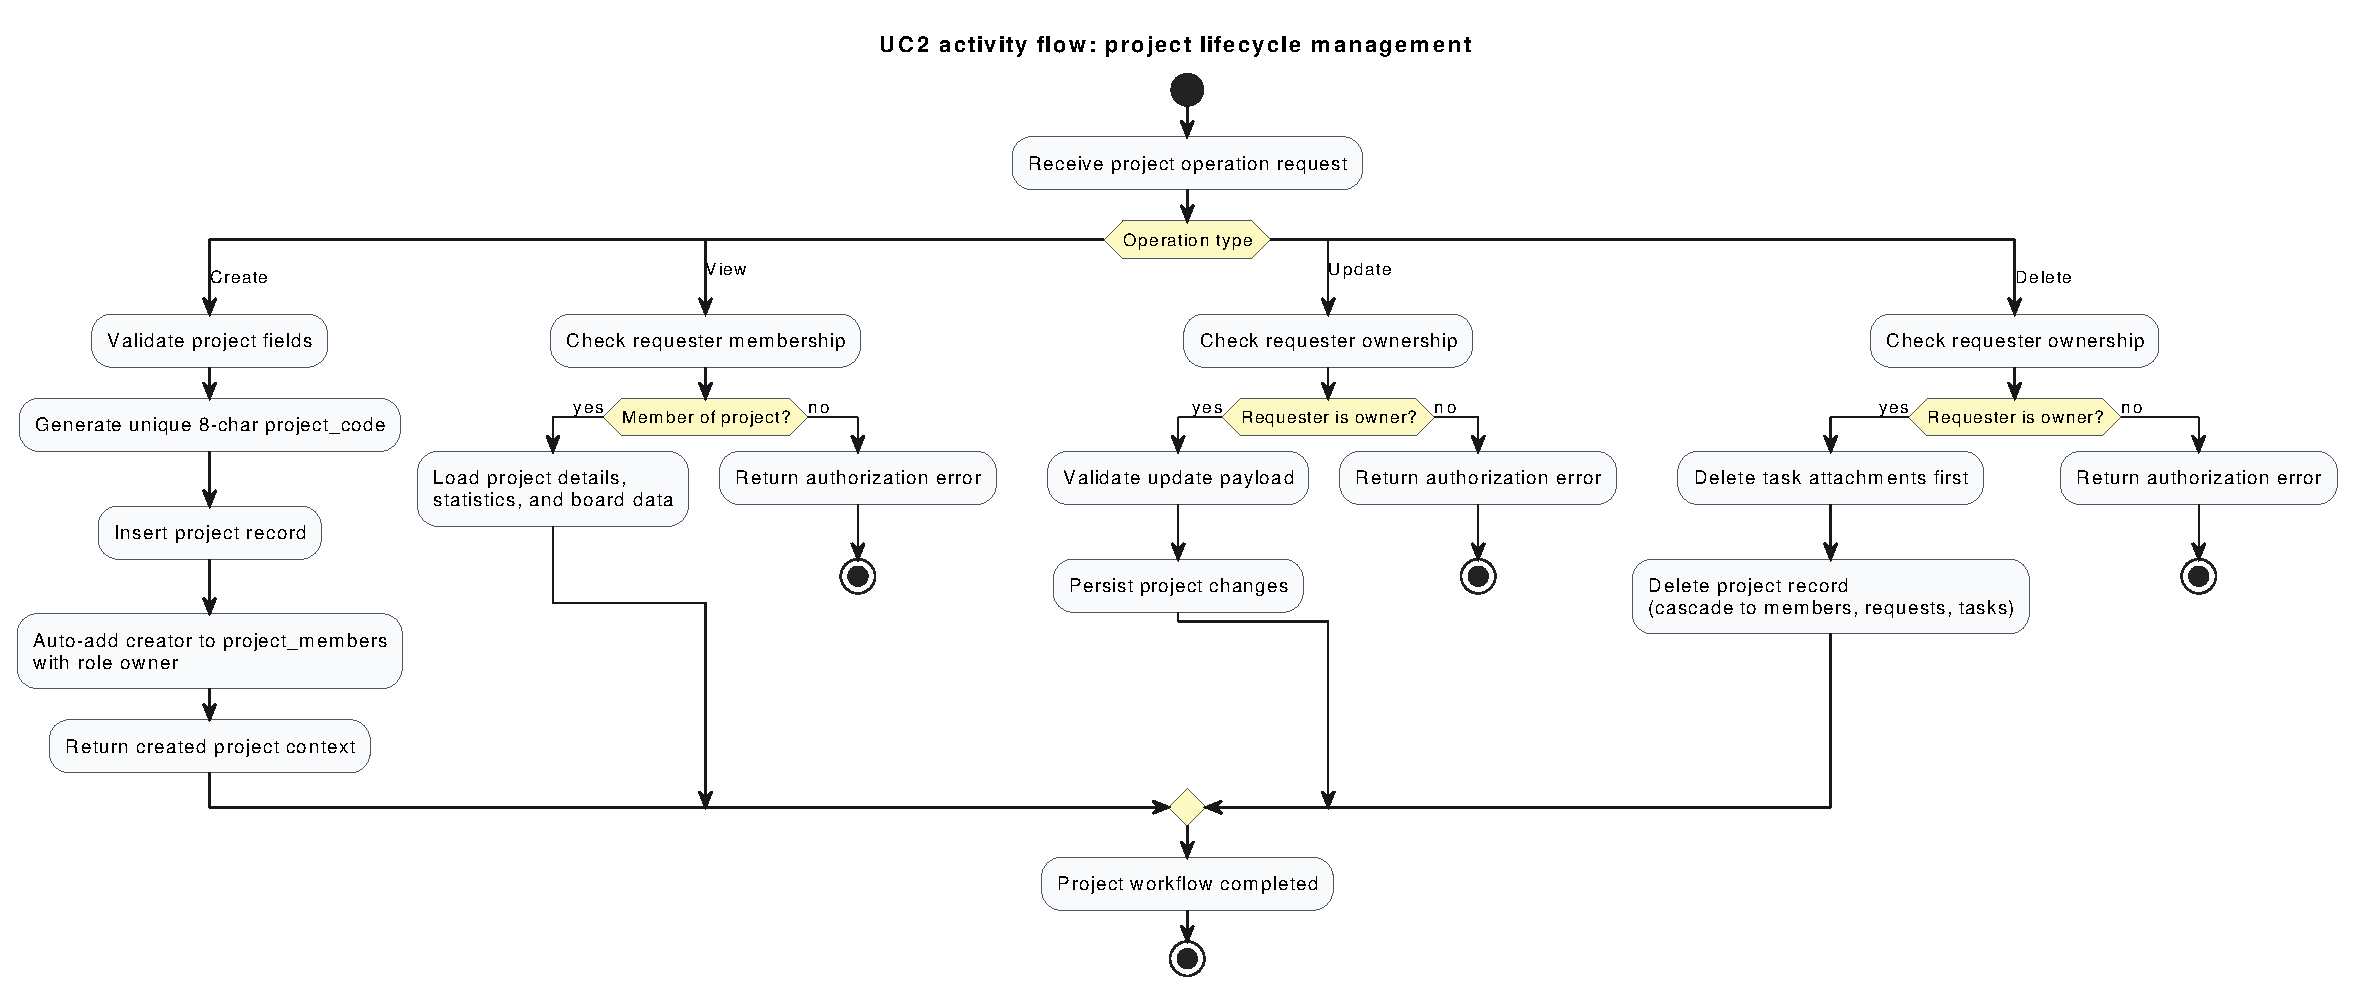
\includegraphics[width=0.90\paperheight,height=0.90\paperwidth,keepaspectratio]{diagrams/generated/uc2-project-flow.pdf}%
}
\caption{UC2 activity flow: project lifecycle management}
\label{fig:uc2-project-flow}
\end{figure}
\end{landscape}
\clearpage

\clearpage
\begin{landscape}
\thispagestyle{landscapefancy}
\begin{figure}[H]
\centering
\makebox[\linewidth][c]{%
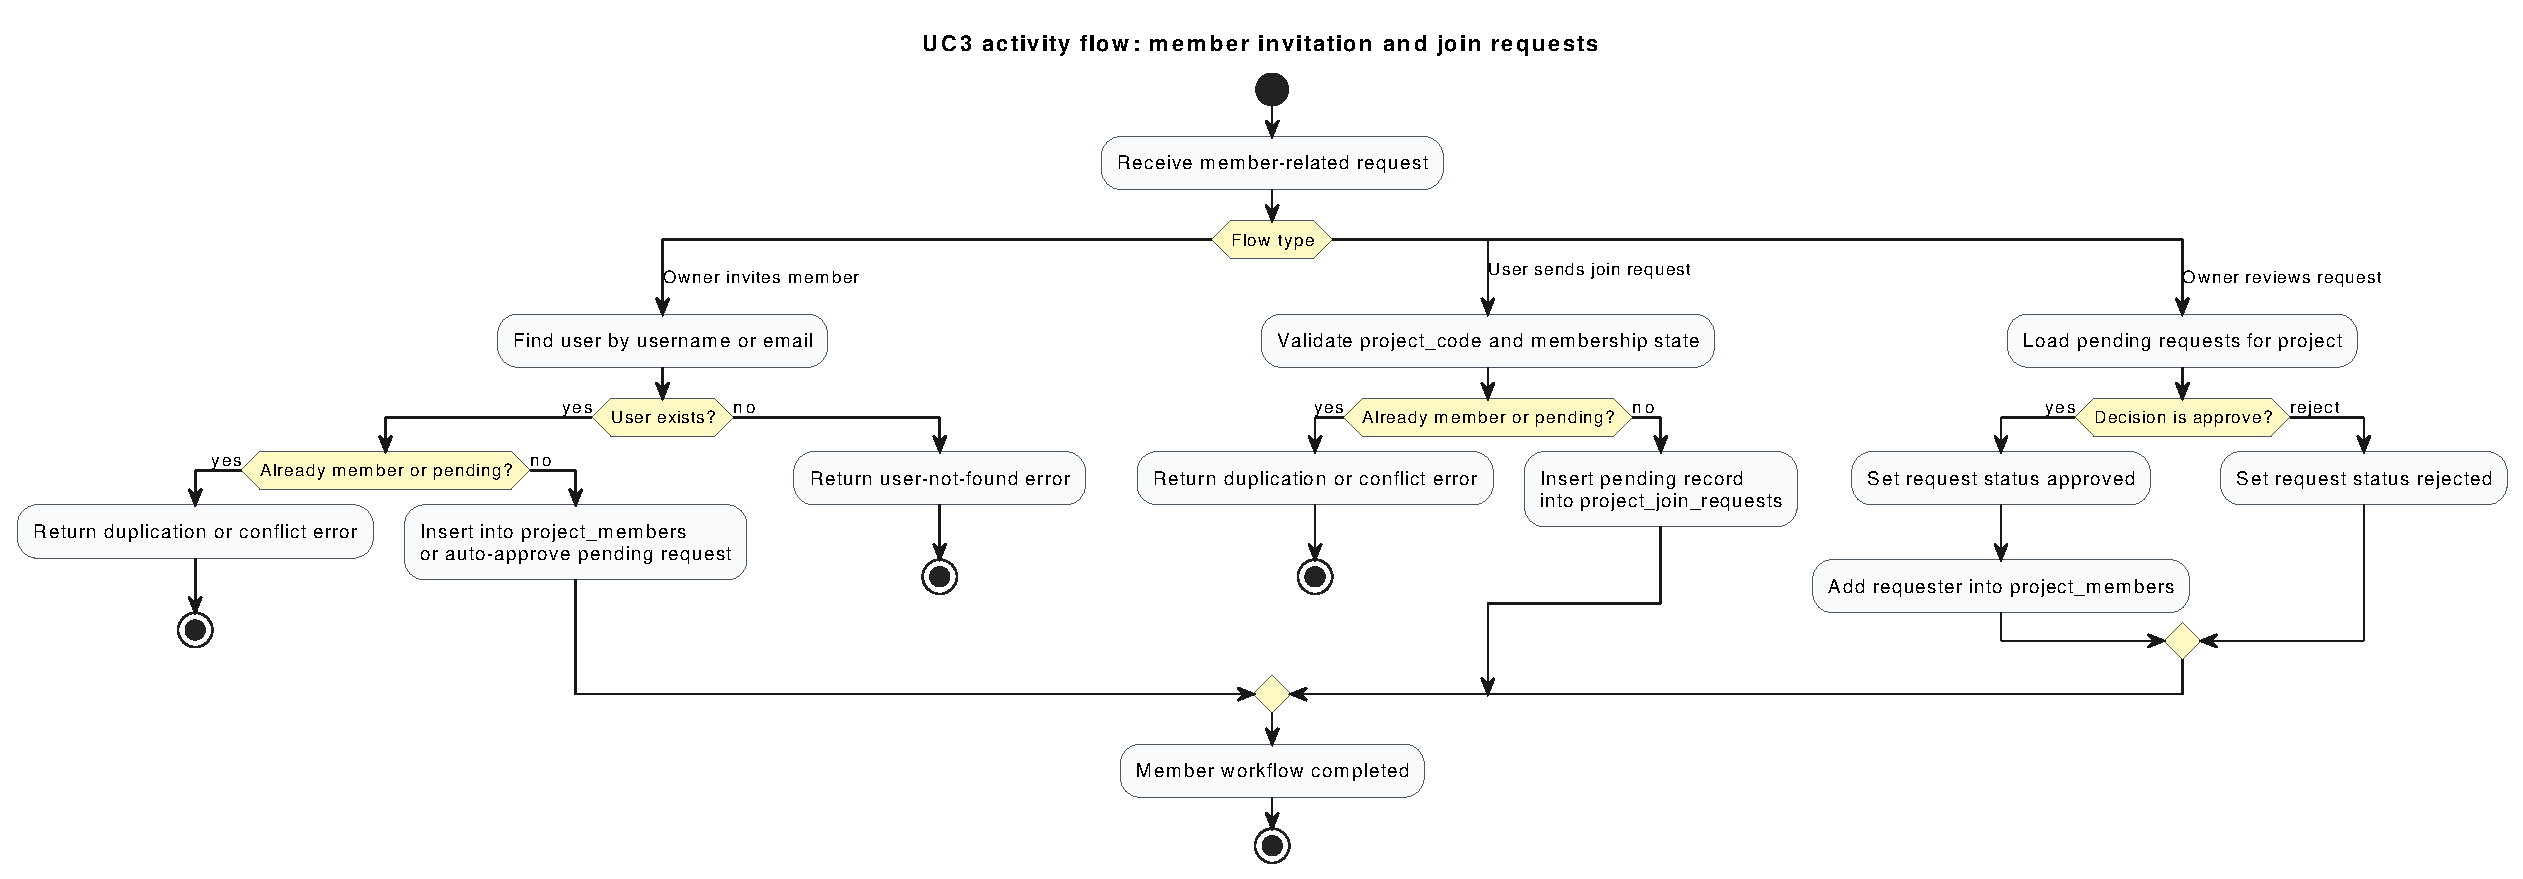
\includegraphics[width=0.90\paperheight,height=0.90\paperwidth,keepaspectratio]{diagrams/generated/uc3-member-flow.pdf}%
}
\caption{UC3 activity flow: member invitation and join requests}
\label{fig:uc3-member-flow}
\end{figure}
\end{landscape}
\clearpage


\subsection{Project Management (UC2)}

Project capabilities include:
\begin{itemize}
    \item Creating a project and auto-registering the creator as owner member.
    \item Generating an 8-character unique project code for sharing.
    \item Owner-only project update and delete operations.
    \item Deleting linked attachments before project deletion to avoid orphan files.
\end{itemize}

\subsection{Member Management (UC3)}

Member collaboration capabilities include:
\begin{itemize}
    \item Owner invites by username or email.
    \item Non-member users request to join via project code.
    \item Owner approves or rejects pending join requests.
    \item Removing a member automatically clears assignments in existing tasks.
\end{itemize}

\subsection{Permission Rules}

The domain logic in \code{includes/member-functions.php} enforces strict project permissions:
\begin{itemize}
    \item Only project owners can add/remove members and process requests.
    \item Members can leave projects, but project owners cannot leave without deleting the project.
\end{itemize}

\screenshotplaceholder{Dashboard with owned and joined projects}{dashboard-project-list.png}
\screenshotplaceholder{Join request review dialog for project owner}{join-request-modal.png}
